\section{Preliminaries}
\label{sec:background}

Distributed collaborative editing systems consider a sequence of characters
replicated on $n$ sites. Each site manages a local copy of the sequence called
local replica. At some moments, the local replica can differ from some other
sites' local replica. Each site can $insert$ and $delete$ characters in the
sequence without any locking mechanism. Then, all sites exchange and deliver
the operations. When any site delivers an insert operation, the state of the
local replica may be different from the state of another replica.

The system is correct if:
\begin{inparaenum}[(i)]
\item It converges i.e. all local replicas of the sequence are equal when the
  system is idle. It corresponds to the eventual consistency
  property~\cite{johnson1975maintenance}.
\item It preserves all partial order relations $\prec$ between characters. If a
  site inserts the character $x$ between the characters $a$ and $b$ ($a \prec x
  \prec b$), this relation is preserved on each sites' replica. It
  corresponds to the property of intention preservation in Operational
  Transformation algorithms~\cite{sun1998achieving} used by Google Docs.
\end{inparaenum}

Let us illustrate this with an example. Assume that all the replicas of a
sequence of characters are equal and that the sequence looks like
$...abcd...$. Consider that a site inserts the character $e$ between $b$ and
$c$ and also consider that at the same moment, another site inserts a character
$f$ between $b$ and $c$. It results in two relations $b \prec e \prec c$ and $b
\prec f \prec c$. Once every site has delivered all the changes on their local
replica, the union of these two relations merges into a partial relation
without any precedence between $e$ and $f$. Consequently, two final states are
possible $abefcd$ and $abfecd$. The role of the sequence CRDTs is to build a
linear extension of the partial order formed by the intentions of all users to
obtain a unique total order.

Variable-size sequence CRDTs encode order relations into identifiers. For
example, the operation $insert(a=10 \prec x \prec b=15)$ can be sent as
$insert(x,12)$. This strategy does not require keeping tombstones, however it
is easy to see that identifiers can grow quickly and significantly degrade the
overall performance of the system. In the worst case, the system requires to
re-balance identifiers implying the use of a consensus algorithm.

In this paper, we focus on keeping the identifiers as small as possible hence
avoiding any costly protocol to re-balance them. Definition~\ref{def:model}
states a document as a set of pairs $(elt, id)$ where $elt$ can be a character
or a line and $id$ are unique immutable identifiers defined on the set of all
possible identifiers $\mathcal{I}$. $\mathcal{I}$ has an order relation $<$
which is dense and strictly totally ordered i.e. if $x,y \in \mathcal{I}$ and
$x < y$ then $\exists z \in \mathcal{I}, z\neq x, z\neq y, x < z <
y$. $alloc(p,q)$ is the allocation strategy function that generates $id \in
\mathcal{I}$. In Definition~\ref{def:id}, we state that an $id$ is a sequence
of numbers, $id_1<id_2$ if $id_1 $ precedes $id_2$ in lexicographic order. This
sequence is an efficient way to represent a dense order.

\begin{Def}[Model of a document]\ \\
A document is a set $\mathcal{D} = \{ (elt, id) \}$ with two operations:
\begin{itemize}
  \item insert($p \in \mathcal{I}$, elt, $q \in
    \mathcal{I}$):- $\mathcal{D} \cup \{(elt,id_{elt})\}$ \\ where
    $id_{elt}=alloc(p,q)$ with $p<id_{elt}<q$
  \item delete($id \in \mathcal{I}$):- $\mathcal{D}/\{(elt,id)\}$
\end{itemize}
\label{def:model}
\end{Def}

\begin{Def}[Variable-size identifier]
  A variable-size identifier $id$ is a sequence of numbers $id=[p_1.p_2\ldots
    p_n]$ which can designate a path in a tree~\footnote{Identifiers should
    include site ID to ensure the uniqueness property. However, for clarity
    purposes and in order to focus on allocation strategy, we did not
    include any site ID in this definition.}.
\label{def:id}
\end{Def}

In Figure~\ref{fig:treeexample}, we represent a document as a tree where each
identifier is a path from the root to a leaf. In this example, each level has a
maximum capacity (arity of the tree node) set to 100. A leaf is an element of
the sequence. For instance, $[10.13]$ is an identifier referencing the element
$b$.  Assume a user wants to insert an element $z$ between two existing
elements identified by $p$ and $q$:
\begin{asparaitem}
\item if $p=[11]$ and $q=[14]$, there is room for insertion. Both identifiers
  $[12]$ and $[13]$ are valid choices for the new element.
\item if $p=[14]$ and $q=[15]$, there is no room at this level. Since the model
  does not have further levels, the allocation function $alloc$ initiates a new
  level. Then, it chooses among this bunch of newly available identifiers:
  between $[14.0]$ and $[14.99]$.
\end{asparaitem}

\begin{figure}[h]
\begin{center}
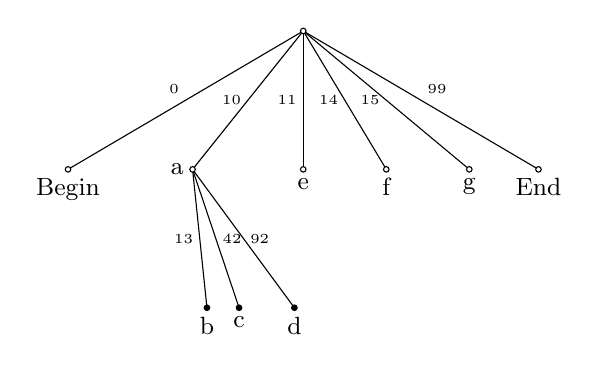
\begin{tikzpicture}[scale=1.0]
\tiny

  
  \draw (0,0) -- node[anchor=south east]{0}  (-85pt, -50pt);
  \draw (0,0) -- node[anchor=south west]{99} ( 85pt, -50pt);

  \draw (0,0) -- node[anchor=east]{10} (-40pt, -50pt);
  \draw (0,0) -- node[anchor=east]{11} (  0pt, -50pt);
  \draw (0,0) -- node[anchor=east]{14} ( 30pt, -50pt);
  \draw (0,0) -- node[anchor=east]{15} ( 60pt, -50pt);

  \draw[fill=white] (0,0) circle (1pt);

\small
  \draw[fill=white] (-85pt, -50pt) node[anchor=north]{Begin} circle (1pt);
  \draw[fill=white] ( 85pt, -50pt) node[anchor=north]{End} circle (1pt);

\tiny
  \draw (-40pt,-50pt) -- node[anchor=east]{13} (-34.8pt, -100pt);
%  \draw (-40pt,-50pt) -- (-30.8pt, -100pt);
  \draw (-40pt,-50pt) -- node[anchor=west]{42} (-23.2pt, -100pt);
%  \draw (-40pt,-50pt) -- (-12.0pt, -100pt);
  \draw (-40pt,-50pt) -- node[anchor=west]{92}(- 3.2pt, -100pt);

\small
  \draw[fill=white] (-40pt, -50pt) node[anchor= east]{\TODO{a}} circle (1pt);
  \draw[fill=white] (  0pt, -50pt) node[anchor= north]{\TODO{e}} circle (1pt);
  \draw[fill=white] ( 30pt, -50pt) node[anchor= north]{\TODO{f}} circle (1pt);
  \draw[fill=white] ( 60pt, -50pt) node[anchor= north]{\TODO{g}} circle (1pt);

  \filldraw[black](-34.8pt, -100pt) node[anchor= north]{\TODO{b}} circle (1pt);
%  \filldraw[black] (-30.8pt, -100pt) node[anchor=north]{23} circle (1pt);
  \filldraw[black](-23.2pt, -100pt) node[anchor= north]{\TODO{c}} circle (1pt);
%  \filldraw[black] (-12.0pt, -100pt) node[anchor=north]{70} circle (1pt);
  \filldraw[black](- 3.2pt, -100pt) node[anchor= north]{\TODO{d}} circle (1pt);

\end{tikzpicture}

\caption{Underlying tree model of a variable-size identifiers sequence CRDT.
  Depth-1 contains four identifiers $[10]$, $[11]$, $[14]$ and $[15]$ labeling
  the elements $a$, $e$, $f$ and $g$ respectively. Also, depth-1 contains the
  bounds of the sequence $\langle [0], Begin \rangle$ and $\langle [99],End
  \rangle$. Depth-2 contains three identifiers $[10.13]$, $[10.42]$, and
  $[10.92]$ labeling $b$, $c$ and $d$ respectively.  }
\label{fig:treeexample}
\end{center}
\end{figure}


\begin{figure*}
\begin{subfigure}[t]{0.47\textwidth}
  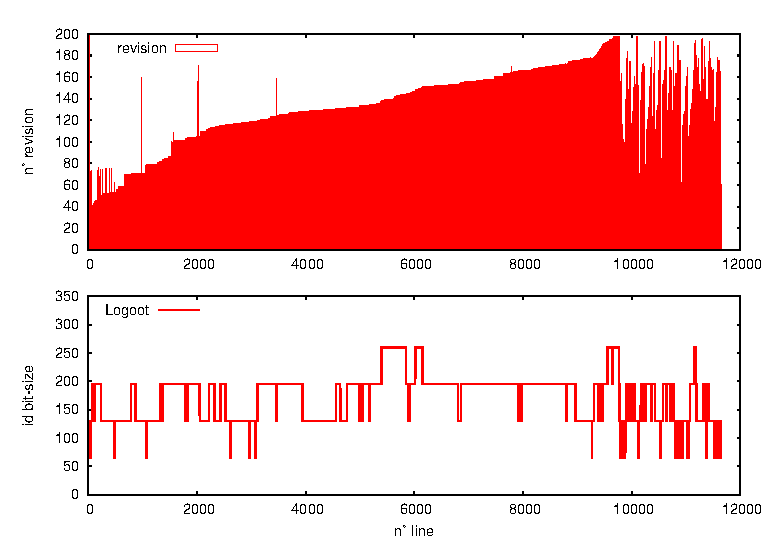
\includegraphics[width=\textwidth]{img/compliant.eps}
  \caption{A page of 12k lines mostly edited at
    the end.}
  \label{im:posteonlyblue}
\end{subfigure}
\hfill
\begin{subfigure}[t]{0.47\textwidth}
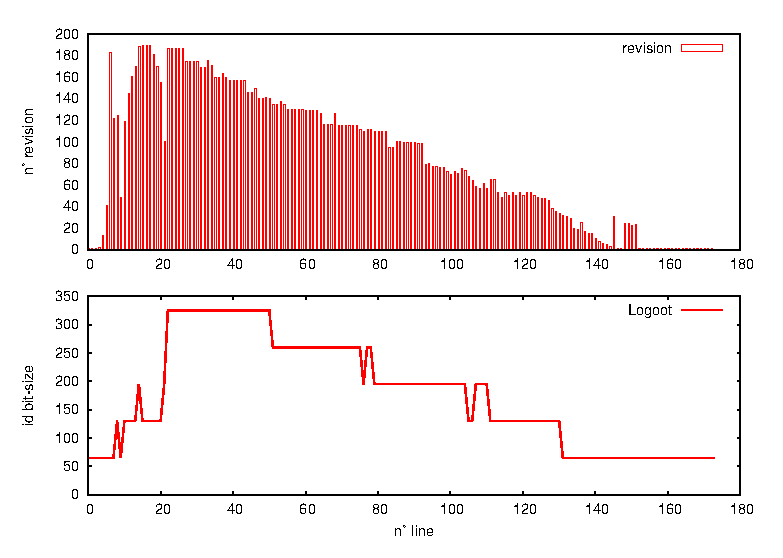
\includegraphics[width=\textwidth]{img/motivating.eps}
\caption{A page of 170 lines mostly edited at the beginning.}
\label{im:didyouknowonlyblue}
\end{subfigure}
\caption{Experiments made on a Wikipedia pages. The top figure shows the
  spectrum of the page (revision number of each line). The bottom figure shows
  the bit-length of the identifier assigned to each line. The allocation
  strategy is $boundary$ from the Logoot approach.}
\end{figure*}

\subsection{Allocation strategies}
The Logoot paper~\cite{weiss2009logoot} already highlighted the importance of
allocation strategies ($alloc$). Indeed, experiments concerned two strategies.
\begin{inparaenum}[(1)]
\item \emph{Random}: randomly choosing between the identifiers of the two
  neighbours. It delivers poor performance because the identifiers quickly
  saturate the space, resulting in the creation of new levels. As consequence,
  the size of identifiers grows quickly.
\item \emph{Boundary}: randomly choosing between the identifiers of the two
  neighbours bounded by a $boundary$ maximum value. The strategy allocates the
  new identifiers closer to their preceding identifier. Of course, it works
  well when the editions are performed right-to-left.
\end{inparaenum}

Figures~\ref{im:posteonlyblue} and~\ref{im:didyouknowonlyblue} show the editing
behaviour and the bit-length of allocated identifiers on two Wikipedia
pages. The top part shows the spectrum associated with the pages. A spectrum
gives an overview of the editing behaviour associated with a page. It gives the
revision number of each line of a document, i.e., the relative date of their
insert operation.  As the left spectrum suggests, most of the insert operations
situates the new elements at the end of the document, i.e., the last lines of
the page are more recent. On the opposite, the second spectrum shows that most
of the insert operations situates the newest elements at the beginning of the
document.  The bottom figures associate the bit-length of the identifier of
each line of the document using the \emph{boundary} strategy. In the first
figure, we consider a page of $12k$ lines. Identifiers do not exceed $256$ bits
and they are well spread between levels $[1-4]$. It leads to a satisfying
average of $169.7$ bits/id. On the contrary, the editing behaviour on the
second document (see figure~\ref{im:didyouknowonlyblue}) that has only 170
lines does not fulfills the right-to-left editing behaviour assumed by the
\emph{boundary} strategy. In this case, we observe, on an existing document,
the worst-case of linear growth of the size of identifiers.  The average
bit-length is $172.25$ bits/id over 5 levels.

\subsection{Issues and motivations}
Most of existing CRDTs' allocation strategies make the assumption of
right-to-left and top-to-bottom editing behaviour. This strong hypothesis
allows better space management but other behaviours may lead to a quick
decrease in performance. Therefore, it makes the distributed collaborative
editor unsafe.

In order to build an efficient distributed collaborative editor based on a
sequence CRDT, we need an adaptive allocation function $alloc$, i.e., an
allocation strategy independent of an editing behaviour. \emph{The
  unpredictability of the editing behaviour makes the allocation of identifiers
  challenging. At any time, the CRDT knows what happened in the past and the
  current operations. Still, inferring the upcoming operations is complex if
  not impossible.}

\begin{Def}[Problem statement]\ \\
Let $\mathcal{D}$ be a document on which $n$ insert operations have been
performed.  Let $\mathcal{I}(\mathcal{D})= \{id |
(\_,id)\in{\mathcal{D}}\}$. The function $alloc(id_p,id_q)$ should provide
identifiers such as:
\begin{center}
$\sum\limits_{id \in \mathcal{I}} { {log_2(id)}\over{n}}$ $< O(n)$
\end{center}
\end{Def}

The problem statement concerns the allocation function $alloc$ which should
have a sub-linear upper-bound in its space complexity. Such function would
greatly improve the current state of art since the document does not require
any additional costly protocol: the average size of identifiers being under an
acceptable bound.
